
In the previous, Working with SourceLocation and SourceManager section, we've learned how source locations, which are an important part of the preprocessor, are represented in Clang. In this section, we will first explain the principle of Clang's preprocessor and lexer, along with their working flow. Then, we'll go into some of the important components in this flow and briefly explain their usage in the code. These will also prepare you for the project in the, Developing custom preprocessor plugins and callbacks section later in this chapter.

\subsubsubsection{6.3.1\hspace{0.2cm}Understanding the role of the preprocessor and lexer in Clang}

The roles and primary actions performed by Clang's preprocessor and lexer, represented by the Preprocessor and Lexer classes respectively, are illustrated in the following diagram:

\hspace*{\fill} \\ %插入空行
\begin{center}
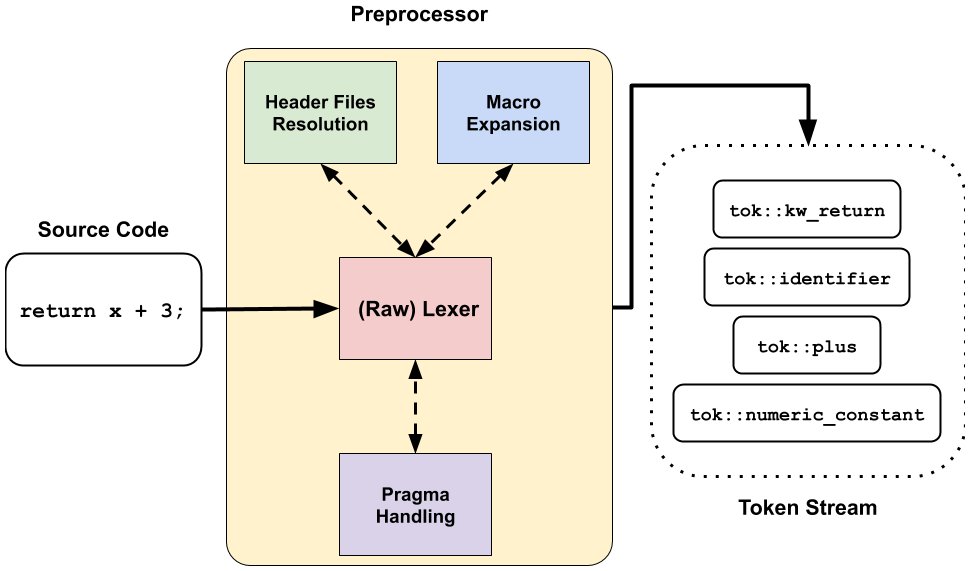
\includegraphics[width=0.8\textwidth]{content/2/chapter6/images/1.png}\\
Figure 6.1 – Role of the Clang preprocessor and lexer
\end{center}

We believe most readers here will be familiar with the concept of a token in the context of the lexer—a substring from the original source code that acts as the minimum building block for semantic reasoning. In some of the traditional compilers, the lexer is responsible for chopping the input source code into a sequence of tokens or a token stream, as shown in the preceding diagram. This token stream will later be fed into the parser to construct the semantic structure.

Implementation-wise, Clang takes a slightly different path from traditional compilers (or those from textbooks): Lexer, employed by Preprocessor, is still the primary performer to cut source code into tokens. However, Lexer keeps its hands off whenever encountering a preprocessor directive (that is, anything that starts with a \#) or a symbol, and relays that task to either the macro expansion, the header file resolver, or pragma handlers that are organized by the Preprocessor. These assisting components inject extra tokens, if needed, into the main token stream, which would eventually be returned back to the user of Preprocessor.

In other words, most consumers of the token stream don't directly interact with Lexer, but with the Preprocessor instances. This makes people call the Lexer class a raw lexer (as shown in the previous diagram), since Lexer by itself only generates a token stream that hasn't been preprocessed. To give you a more concrete idea of how to use Preprocessor to retrieve a token (stream), the following simple code snippet has been provided. This shows a way to get the next token from the source code currently processing it:

\begin{lstlisting}[style=styleCXX]
Token GetNextToken(Preprocessor &PP) {
	Token Tok;
	PP.Lex(Tok);
	return Tok;
}
\end{lstlisting}

As you might have guessed, Token is the class representing a single token in Clang, which we're going to introduce shortly in the next paragraph.

\subsubsubsection{6.3.2\hspace{0.2cm}Understanding Token}

The Token class is the representation of a single token, either from the source code or a virtual one that served a special purpose. It is also used extensively by the preprocessing/lexing framework, just like SourceLocation that we introduced earlier. Thus, it is designed to be very concise in memory and trivially copyable as well.

For the Token class, there are two things we want to highlight here, as follows:

\begin{enumerate}
\item Token kind tells you what this token is.
\item Identifier represents both language keywords and arbitrary frontend tokens (a function name, for example). Clang's preprocessor used a dedicated IdentifierInfo class to carry extra identifier information, which we're going to cover later in this section.
\end{enumerate}

\hspace*{\fill} \\ %插入空行
\noindent
\textbf{Token kind}

The token kind tells you what this Token is. Clang's Token is designed to represent not just concrete, physical-language constructions such as keywords and symbols, but also virtual concepts that are inserted by the parser in order to encode as much information as possible using a single Token. To visualize the token stream's token kinds, you can use the following command-line option:

\begin{tcblisting}{commandshell={}}
$ clang -fsyntax-only -Xclang -dump-tokens foo.cc
\end{tcblisting}

foo.cc has the following content:

\begin{lstlisting}[style=styleCXX]
namespace foo {
	class MyClass {};
}
foo::MyClass Obj;
\end{lstlisting}

This is the output of the preceding command:

\begin{tcblisting}{commandshell={}}
namespace 'namespace' [StartOfLine] Loc=<foo.cc:1:1>
identifier 'foo' [LeadingSpace] Loc=<foo.cc:1:11>
l_brace '{' [LeadingSpace] Loc=<foo.cc:1:15>
class 'class' [StartOfLine] [LeadingSpace] Loc=<foo.
cc:2:3>
identifier 'MyClass' [LeadingSpace] Loc=<foo.cc:2:9>
l_brace '{' [LeadingSpace] Loc=<foo.cc:2:17>
	r_brace '}' Loc=<foo.cc:2:18>
semi ';' Loc=<foo.cc:2:19>
r_brace '}' [StartOfLine] Loc=<foo.cc:3:1>
identifier 'foo' [StartOfLine] Loc=<foo.cc:5:1>
coloncolon '::' Loc=<foo.cc:5:4>
identifier 'MyClass' Loc=<foo.cc:5:6>
identifier 'Obj' [LeadingSpace] Loc=<foo.cc:5:14>
semi ';' Loc=<foo.cc:5:17>
eof '' Loc=<foo.cc:5:18>
\end{tcblisting}

The highlighted parts are the token kinds for each token. The full list of token kinds can be found in clang/include/clang/Basic/TokenKinds.def. This file is a useful reference to know the mapping between any language construction (for example, the return keyword) and its token kind counterpart (kw\_return).

Although we can't visualize the virtual tokens—or annotation tokens, as they are called in Clang's code base—we will still explain these using the same example as before. In C++, :: (the coloncolon token kind in the preceding directive) has several different usages. For example, it can either be for namespace resolution (more formally called scope resolution in C++), as shown in the code snippet earlier, or it can be (optionally) used with the new and delete operators, as illustrated in the following code snippet:

\begin{lstlisting}[style=styleCXX]
int* foo(int N) {
	return ::new int[N]; // Equivalent to 'new int[N]'
}
\end{lstlisting}

To make the parsing processing more efficient, the parser will first try to resolve whether the coloncolon token is a scope resolution or not. If it is, the token will be replaced by an annot\_cxxscope annotation token.
 
Now, let's see the API to retrieve the token kind. The Token class provides a getKind function to retrieve its token kind, as illustrated in the following code snippet:

\begin{lstlisting}[style=styleCXX]
bool IsReturn(Token Tok) {
	return Tok.getKind() == tok::kw_return;
}
\end{lstlisting}

However, if you're only doing checks, just like in the preceding snippet, a more concise function is available, as illustrated here:

\begin{lstlisting}[style=styleCXX]
bool IsReturn(Token Tok) {
	return Tok.is(tok::kw_return);
}
\end{lstlisting}

Though many times, knowing the token kind of a Token is sufficient for processing, some language structures require more evidence to judge (for example, tokens that represent a function name, in which case the token kind, identifier, is not as important as the name string). Clang uses a specialized class, IdentifierInfo, to carry extra information such as the symbol name for any identifier in the language, which we're going to cover in the next paragraph.

\hspace*{\fill} \\ %插入空行
\noindent
\textbf{Identifier}

Standard C/C++ uses the word identifier to represent a wide variety of language concepts, ranging from symbol names (such as function or macro names) to language keywords, which are called reserved identifiers by the standard. Clang also follows a similar path on the implementation side: it decorates Token that fit into the language's standard definition of an identifier with an auxiliary IdentifierInfo object. This object encloses properties such as the underlying string content or whether this identifier is associated with a macro function. Here is how you would retrieve the IdentifierInfo instance from a Token type variable Tok:

\begin{lstlisting}[style=styleCXX]
IdentifierInfo *II = Tok.getIdentifierInfo();
\end{lstlisting}

The preceding getIdentifierInfo function returns null if Tok is not representing an identifier by the language standard's definition. Note that if two identifiers have the same textual content, they are represented by the same IdentifierInfo object. This comes in handy when you want to compare whether different identifier tokens have the same textual contents.

Using a dedicated IdentifierInfo type on top of various token kinds has the following advantages:

\begin{itemize}
\item For a Token with an identifier token kind, we sometimes want to know if it has been associated with a macro. You can find this out with the IdentifierInfo::hasMacroDefinition function.

\item For a token with an identifier token kind, storing underlying string content in auxiliary storage (that is, the IdentifierInfo object) can save a Token object's memory footprint, which is on the hot path of the frontend. You can retrieve the underlying string content with the IdentifierInfo::getName function.

\item For a Token that represents language keywords, though the framework already provides dedicated token kinds for these sorts of tokens (for example, kw\_return for the return keyword), some of these tokens only become language keywords in later language standards. For example, the following snippet is legal in standards before C++11:
\begin{lstlisting}[style=styleCXX]
void foo(int auto) {}
\end{lstlisting}

\item You could compile it with the following command:
\begin{tcblisting}{commandshell={}}
$ clang++ -std=c++03 -fsyntax-only …
\end{tcblisting}
If you do so, it won't give you any complaint, until you change the preceding -std=c++03 standard into -std=c++11 or a later standard. The error message in the latter case will say that auto, a language keyword since C++11, can't be used there. To give the frontend have an easier time judging if a given token is a keyword in any case, the IdentifierInfo object attached on keyword tokens is designed to answer if an identifier is a keyword under a certain language standard (or language feature), using the IdentifierInfo::isKeyword(…) function, for example, whereby you pass a LangOptions class object (a class carrying information such as the language standard and features currently being used) as the argument to that function.

\end{itemize}

In the next sub-section, we're going to introduce the last important Preprocessor concept of this section: how Preprocessor handles macros in C-family languages.

\subsubsubsection{6.3.3\hspace{0.2cm}Handling macros}

Implementations for macros of C-family languages are non-trivial. In addition to challenges on source locations as we introduced earlier—how do we carry source locations of both the macro definitions and the place they're expanded—the ability to re-define and undefine a macro name complicates the whole story. Have a look at the following code snippet for an example of this:

\begin{lstlisting}[style=styleCXX]
#define FOO(X) (X + 1)
return FOO(3); // Equivalent to "return (3 + 1);"
#define FOO(X) (X - 100)
return FOO(3); // Now this is equivalent to "return (3 - 100);"
#undef FOO
return FOO(3); // "FOO(3)" here will not be expanded in
			   //preprocessor
\end{lstlisting}

The preceding C code showed that the definition of FOO (if FOO is defined) varies on different lexical locations (different lines).

\begin{tcolorbox}[colback=blue!5!white,colframe=blue!75!black, fonttitle=\bfseries,title=Local versus Module macros]
\hspace*{0.7cm}C++20 has introduced a new language concept called Module. It resembles the modularity mechanisms in many other object-oriented languages such as Java or Python. You can also define macros in a Module, but they work slightly differently from the traditional macros, which are called local macros in Clang. For example, you can control the visibility of a Module macro by using keywords such as export. We only cover local macros in this book.
\end{tcolorbox}

To model this concept, Clang has constructed a system to record the chain of definitions and un-definitions. Before explaining how it works, here are three of the most important components of this system:

\begin{enumerate}
\item MacroDirective: This class is the logical representation of a \#define or a \#undef statement of a given macro identifier. As shown in the preceding code example, there can be multiple \#define (and \#undef) statements on the same macro identifier, so eventually these MacroDirective objects will form a chain ordered by their lexical appearances. To be more specific, the \#define and \#undef directives are actually represented by subclasses of MacroDirective, DefMacroDirective, and UndefMacroDirective, respectively.

\item MacroDefinition: This class represents the definition of a macro identifier at the current time point. Rather than containing the full macro definition body, this instance is more like a pointer pointing to different macro bodies, which are represented by the MacroInfo class that will be introduced shortly, upon resolving a different MacroDirective class. This class can also tell you the (latest) DefMacroDirective class that defines this MacroDefinition class.

\item MacroInfo: This class contains the body, including tokens in the body and macro arguments (if any) of a macro definition.

\end{enumerate}

Here is a diagram illustrating the relationship of these classes in regard to the sample code earlier:

\hspace*{\fill} \\ %插入空行
\begin{center}
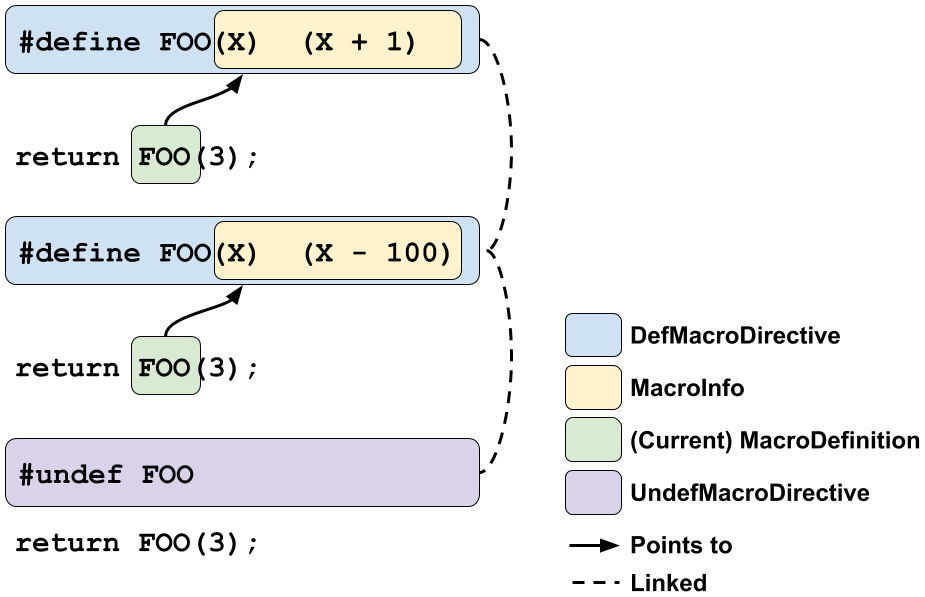
\includegraphics[width=0.9\textwidth]{content/2/chapter6/images/2.png}\\
Figure 6.2 – How different C++ classes for a macro are related to the previous code example
\end{center}

To retrieve the MacroInfo class and its MacroDefinition class, we can use the following Preprocessor APIs, as follows:

\begin{lstlisting}[style=styleCXX]
void printMacroBody(IdentifierInfo *MacroII, Preprocessor &PP)
{
	MacroDefinition Def = PP.getMacroDefinition(MacroII);
	MacroInfo *Info = Def.getMacroInfo();
	…
}
\end{lstlisting}

The IdentifierInfo type argument, MacroII, shown in the preceding code snippet, represents the macro name. To further examine the macro body, run the following code:

\begin{lstlisting}[style=styleCXX]
void printMacroBody(IdentifierInfo *MacroII, Preprocessor &PP)
{
	…
	MacroInfo *Info = Def.getMacroInfo();
	for(Token Tok : Info->tokens()) {
		std::cout << Tok.getName() << "\n";
	}
}
\end{lstlisting}

From this section, you've learned the working flow of Preprocessor, as well as two important components: the Token class and the sub-system that handles macros. Learning these two gives you a better picture of how Clang's preprocessing works and prepares you for the Preprocessor plugin and custom callbacks development in the next section.





























